\section*{Introduction}

\textbf{Motivation:} Single-cell RNA-seq is a promising technique that profiles transcriptomes over a plethora of cell types. By measuring individual cells, rather than averaged tissue types, scRNA-seq can uncover biological mechanisms that is not observed by the average behaviors of a bulk of cells  \citep{wang2017vasc}. However, despite improvements in measuring technologies, factors including amplification bias, cell cycle effects \citep{buettner2015computational}, etc. lead to substantial noise in scRNA-seq experiments. The low RNA capture rate leads to failure of detection of an expressed gene resulting in a ``false" zero count observation, defined as dropout event; which potentially corrupts the underlying biological signal \cite{eraslan2018single}. One such scRNA-seq data set is from the 10x genomics project that  profiles 1.3 M embroynic brain cells of mice. It represents cells from cortex, hippocampus and subventricular zone of two mice at 18 days post conception which is an invaluable resource to study gene dynamics during an important development stage, however, the corruption induced by dropout events compromises our ability to use analytical techniques to extract meaningful patterns. 

Current approaches for scRNA-seq denoising / imputation rely on using the correlation structure of single-cell gene expression data, leveraging similarities between cells and/or genes that does not scale well; or has explicit / implicit linearity assumption that may miss complex non-linear patterns \citep{eraslan2018single}. Deep-learning auto-encoders can learn the underlying complex manifold, that represents the biological processes and/or cellular states and utilize that to reduce the high dimensional data space to significantly lower dimensions \citep{moon2017manifold}. However, using an auto-encoder as is may fail due to the noise model not being adapted to typical scRNA-seq noise. One such autoencoder DCA -- deep count autoencoder facilitates non-linear embedding of cells and uses scRNA-seq data specific loss function based on negative binomial count distributions which offers adaptive learning and encoding of the data manifold \citep{eraslan2018single}. Thus, we utilize DCA to denoise and reduce the dataset and then apply the classical decision tree algorithms to learn if gene expression dynamics can infer different cell types.

\textbf{Problem definition:} Given expression of X genes across m cell types, we denoise and reduce the data set to X' gene expression of m cell types, expecting $n(X') \leq n(X)$ by using the DCA autoencoder. We then apply the decision tree classifier on X' (genes expressions) to learn the m classes (cell types). We also apply the decision tree algorithm on the raw data to see if the encoded X' actually results in improved accuracy.

\section*{Solution}

\subsection*{Data source}
We are using Single Cell Gene Expression Dataset by Cell Ranger 1.3.0 from the 10x Genomics project that provides 1.3 Million Brain Cells from E18 Mice which consists of cells from cortex, hippocampus and subventricular zone of two E18 mice. The data was retrieved from \href{https://support.10xgenomics.com/single-cell-gene-expression/datasets/1.3.0/1M_neurons}{\textcolor{blue}{support.10xgenomics.com}}.

\begin{figure*}
\begin{framed}
\begin{minipage}{\linewidth}
\begin{minipage}[t]{0.48\linewidth}
\vspace{0pt}
\textsf{a)}\\
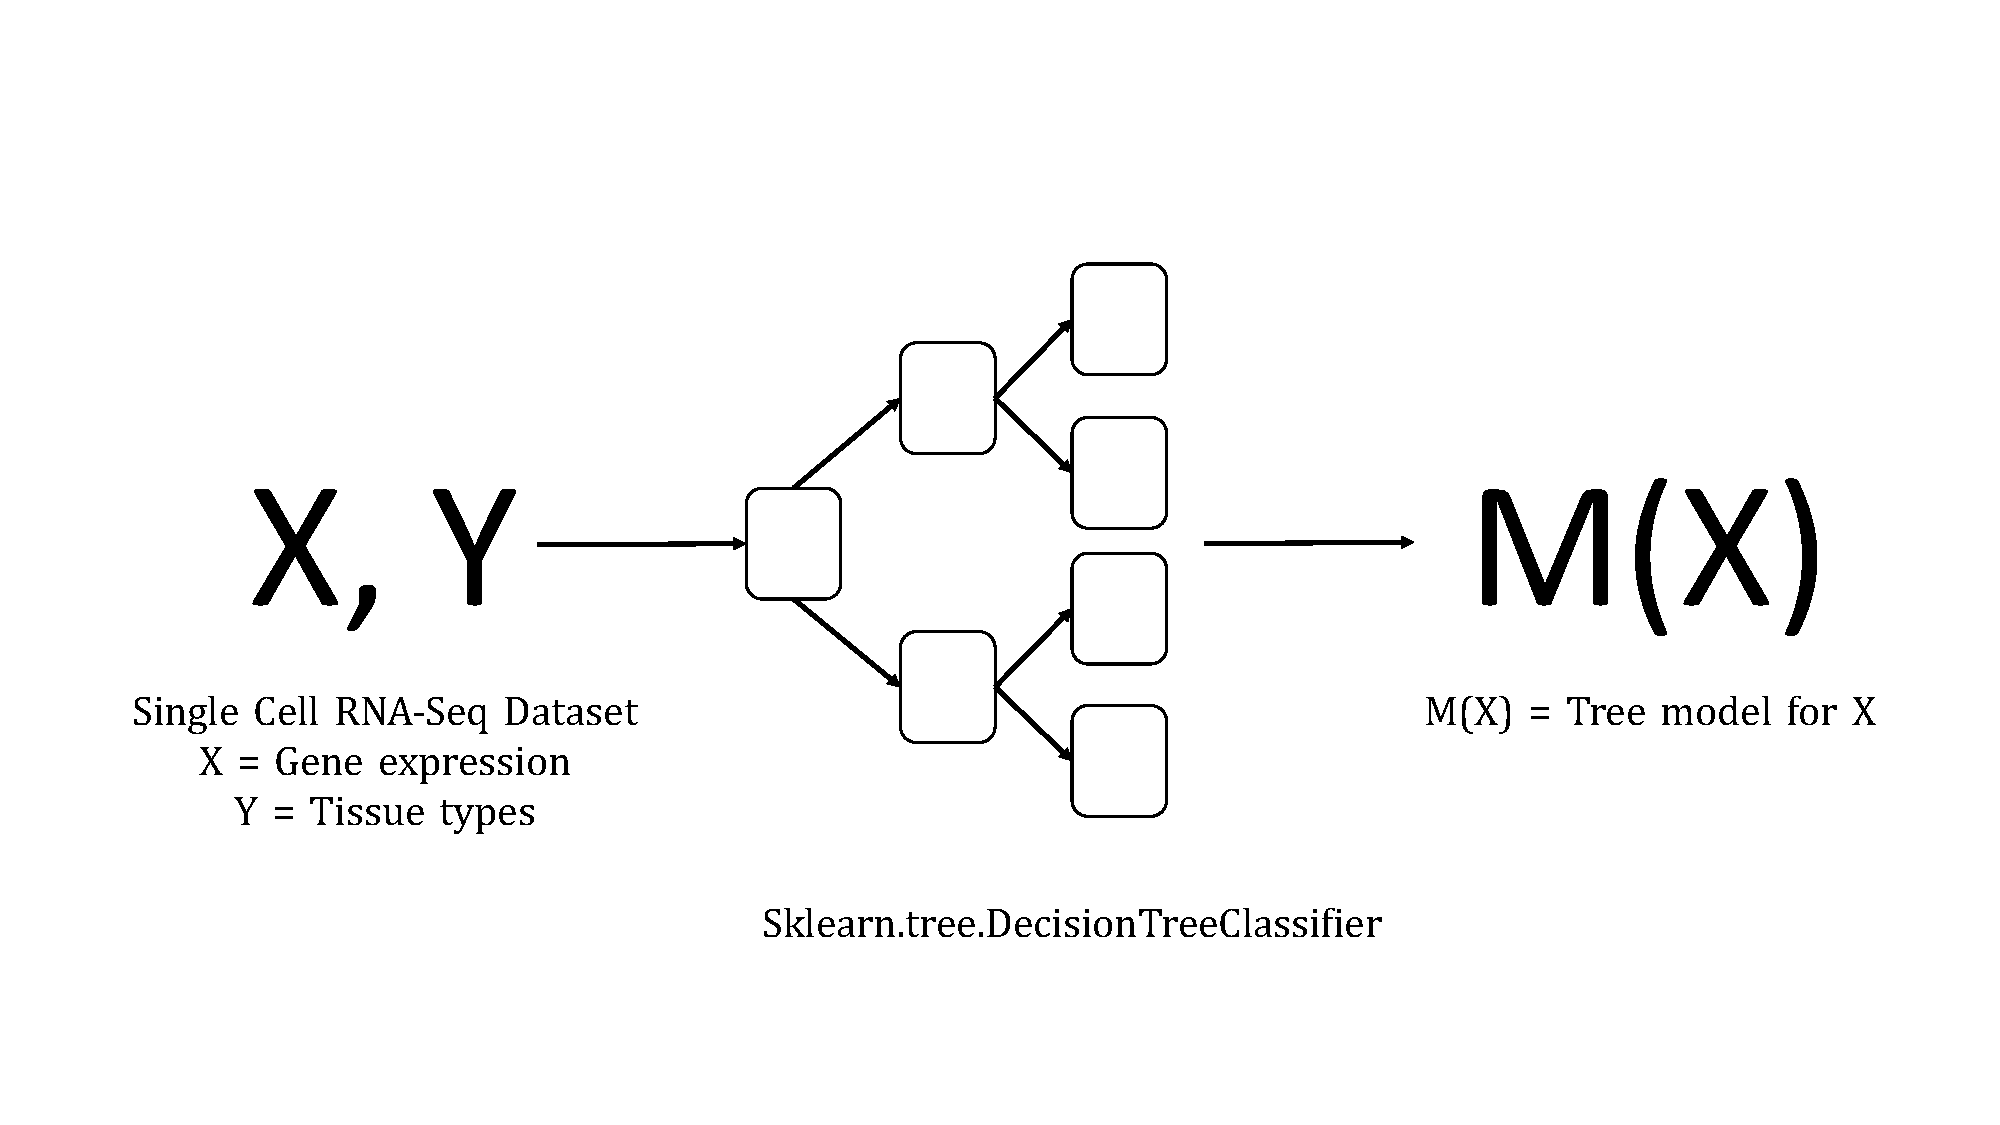
\includegraphics[width=\linewidth]{without_autoencoding.pdf}
\end{minipage}
\begin{minipage}[t]{0.48\linewidth}
\vspace{0pt}
\textsf{b)}\\
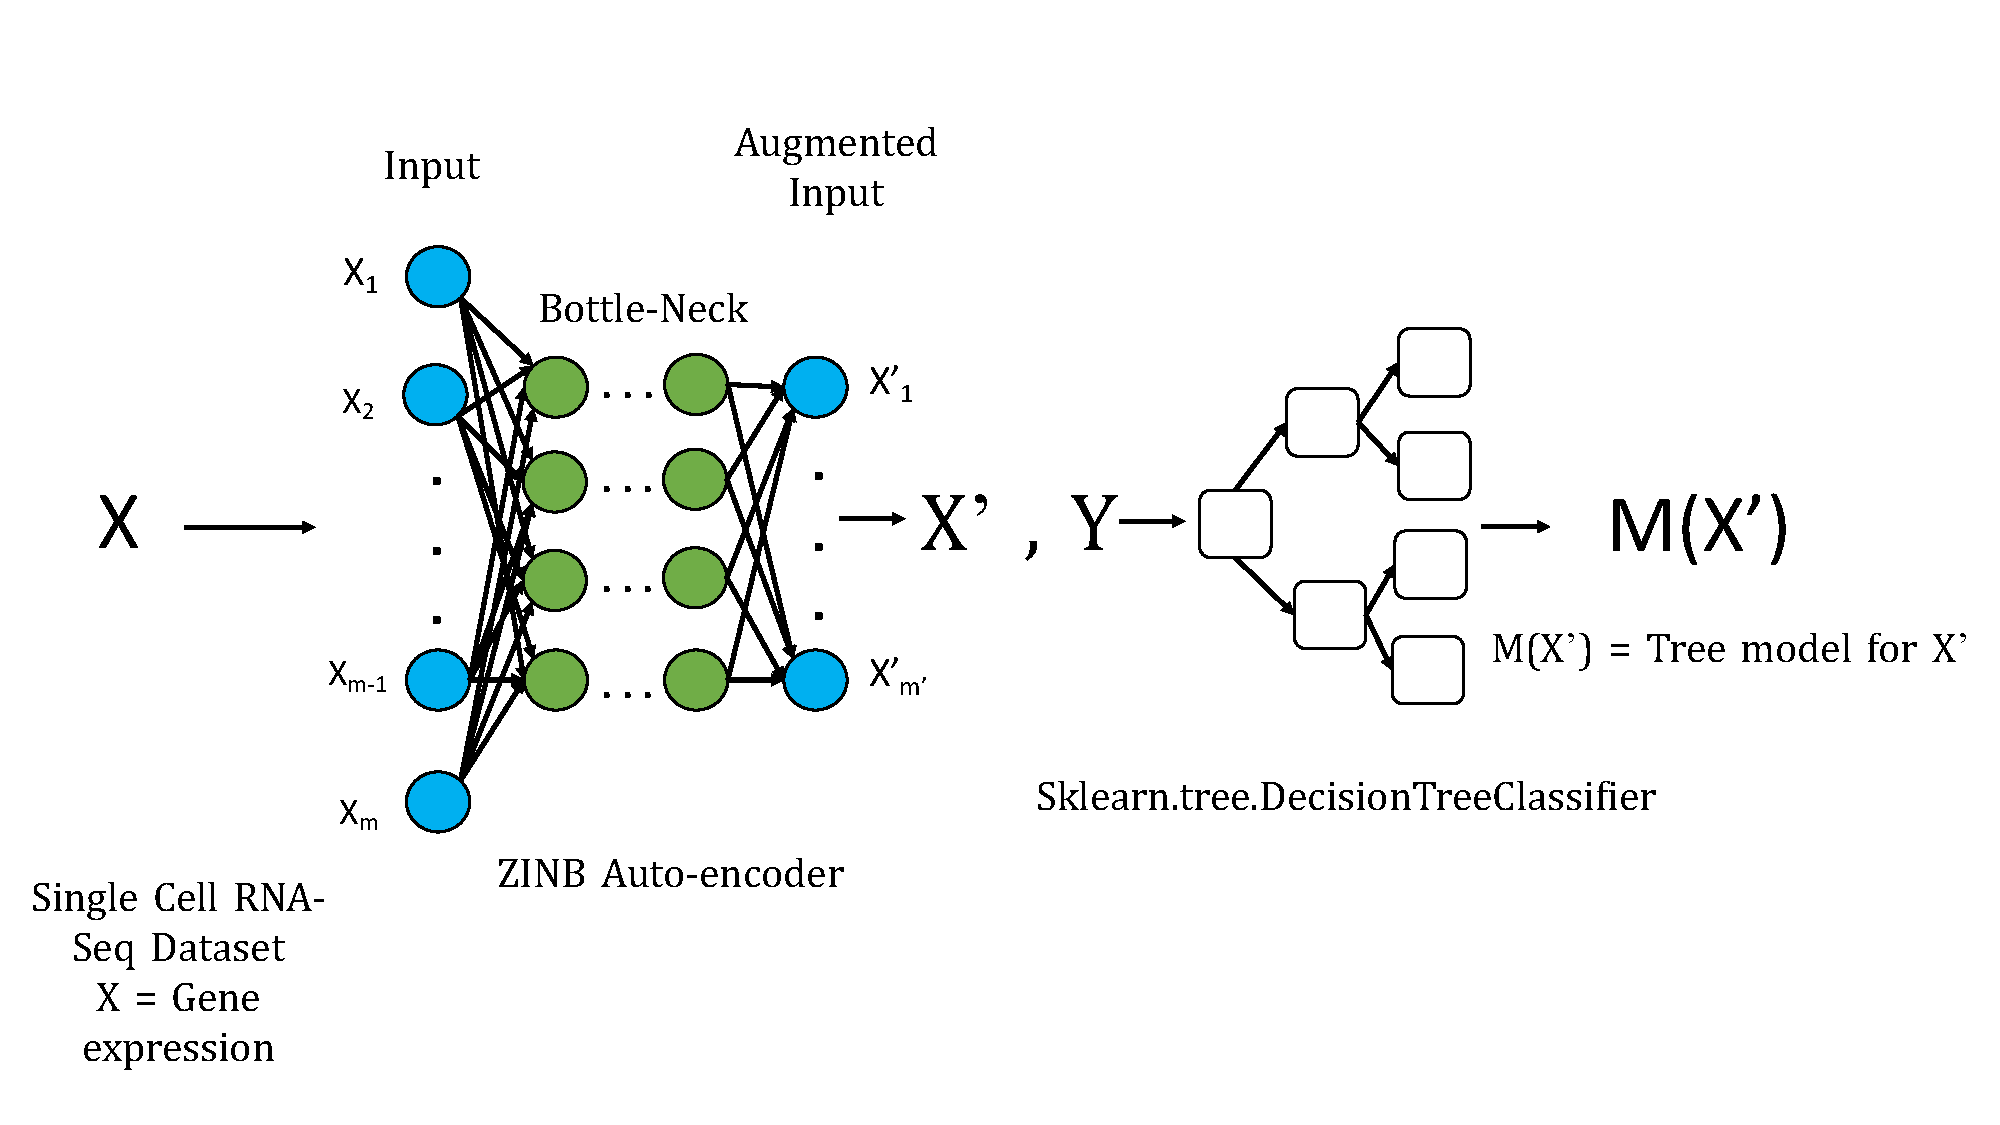
\includegraphics[width=\linewidth]{with_autoencoding.pdf}
\end{minipage}
\end{minipage}
\caption{a) In the first analysis without any denoising, the single cell data will be supplied as is to a sklearn decision tree algorithm. b) In the second analysis, the single cell data will be denoised using the ZINB DCA autoencoder and then the learned manifold X$^{'}$ will be supplied to the sklearn decision tree algorithm.}
\end{framed}
\label{fig1}
\end{figure*}

\subsection*{Proposed Pipeline}
We will proceed with two phases of analysis as shown in figure~1. The first phase would include using the single cell data 'as-is' ($X$, $Y$) and learn if there exists a non-linear combination of gene expression $M(X)$ that can differentiate between the three class labels ($Y$) : \textit{cortex}, \textit{hippo-campus} and  \textit{sub-ventricular zone}. We will be utilizing the decision tree classifier -- \textit{sklearn.tree.DecisionTreeClassifier} provided by sci-kit learn package in Python. We will use sklearn.model\_selection to perform the 10-fold cross-validation strategy and evaluate the performance of the decision tree model.

Next, we will use the zero-inflated negative binomial (ZINB) DCA auto-encoder \citep{eraslan2018single} to first denoise the single cell data ($X$) and see if we can learn the manifold of the data, as claimed by the authors of this method. The augmented data $X'$ will then be given to a similar setup of decision-tree learning with 10-fold cross validation to learn the three cell types. Our final objective would be to report any improvement in performance, followed by deeper insight on to why/why didn't the auto-encoding worked. Our expectation is that the augmented data $X'$ should work better as it uses zero-inflated negative binomial distribution that can model highly sparse and over-dispersed data \citep{eraslan2018single} which makes it very suitable for single-cell RNA-seq.

\subsection*{Preliminary results}
Before applying the ZINB DCA auto-encoder, we established the performance of normalized single-cell gene expression profiles to predict cell types. For this purpose we used head and neck cancer single-cell data-set (GSE103322) \citep{puram2017single} that profiled 23686 genes across 5902 single cells obtained from head and neck region of 18 patients. This data-set contains both normal and cancer samples, where the normal samples come from a patient's non-metastasized areas. We only used normal samples, reducing our sample size to 3363 containing :  B-cell(138), Dendritic(51), Endothelial(260),  Fibroblast(1440), Macrophage(98), Mast(120), Myocyte(19) and T cell(1237). 

\begin{table}[!hbtp]
\begin{tabular}{|c|c|c|c|c|c|c|c|c|c|}
\hline
\textbf{1} & \textbf{2} & \textbf{3} & \textbf{4} & \textbf{5} & \textbf{6} & \textbf{7} & \textbf{8} & \textbf{9} & \textbf{10} \\\hline
0.97 & 0.96 & 0.98 & 0.98 & 0.97 & 0.98 & 0.97 & 0.97 & 0.89 & 0.87 \\\hline
\end{tabular}
\caption{Accuracy over 10-fold cross validation.}
\end{table}  

The task at hand was to model the 8 cell-types as a non-linear combination of gene-expression using decision tree learning. We utilized \textit{sklearn.tree.DecisionTreeClassifier} for the task using default values of all parameters except \texttt{min\_samples\_split} which was set to 20 and \texttt{min\_samples\_leaf} which was set to 5. The single-cell data was transformed using the \textit{sklearn.preprocessing.StandardScaler} transformation. We utilized the 10-fold cross-validation strategy, using stratified partition of cell-types, to measure the accuracy of our decision tree model. Table~1 shows accuracy for all 10 runs using 9/10th data as training and the rest 1/10th as testing, using different subset every-time.

Interestingly, this single-cell data can already do very well. Also, the number of decision tree nodes used to accomplish such accuracy was a modest 61 nodes, which means only a handful genes out of 23K genes can reliably predict the 8 cell-types. We rationaled that the high accuracy could be because of the imbalance in class distribution, however, Fibroblast and T-cells are quite balanced and the decision-tree was able to reliably distinguish between the two cell types. 

While genes being able to distinguish cell types is not surprising, recently, \citet{karaiskos2017drosophila} used ISH (In-situ hybridization) stains of 84 genes to perfectly classify over 3000 cell locale in Drosophila embryo. However, single-cell, due to its noisy nature has not been thought to have the ability to be good at classifying cell-types. It would be interesting to see how other single-cell data-sets do in this scenario and how much can the performance improve after denoising. Unfortunately, the head-and-neck cancer single cell data-set does not offer raw data for denoising, but our final steps include considering methods to un-normalize the single-cell data and try other single-cell data with availability of the raw samples.  Another noticeable peculiarity was a major drop in accuracy for the last two runs. We are yet to investigate on that issue.